\documentclass[12pt]{cnihepsop}
\title{Module assembly: Gluing of Hybrid}
\date{\today}
\author{Matthew Kurth, Yuzhen Yang, Xin Shi}
\approved{Xin Shi}
\sopid{101}
\sopversion{v4}
\sophistory{ 
    \begin{tabular}{|c|c|c|c|} \hline %
        Revision & Date & Editor & Contents \\
        \hline 
        v1 & 2018.02.02 &  Yuzhen Yang and Xin Shi  &  Created document \\
        v2 & 2018.02.08 &  Yuzhen Yang &  Drafted the framework \\
        v3 & 2018.03.20 &  Xin Shi &  Add revision section \\
    	v4 & 2018.03.29 & Matthew Kurth & Add to procedure\\ 
        \hline 
    \end{tabular}% Date & Editor & Contents \\
}

\sopabstract{Describes the procedures to glue ASICs on a strip-module hybrid using the Nordson EFD Dispensing Robot. 
The procedure takes place in the IHEP Hall 3 clean room.}


\begin{document}

\maketitle

%------------------------------------------------------------------
\section{Scope}
This is a regular part in the manufacturing process of silicon-strip module assembly at IHEP.

%------------------------------------------------------------------
\section{Purpose}
Hybrids are assemblied in-situ with both surface mount device (SMD) components and ASICs. The pre-tested ASICs(ABCStars) are glued onto the SMD components which are on a panel. 

%------------------------------------------------------------------
\section{Definitions}
\begin{itemize}
\item Fiducials: The level of panel, the high of pickup tool...
\item Front panel: 
  \begin{enumerate}
    \item In the main front panel only two step buttons are enabled at a time: the ``start'' button and the emergency button. 
    %\item 
  \end{enumerate}
\end{itemize}


%------------------------------------------------------------------
%\section{Responsibilities}

%------------------------------------------------------------------
\section{Equipment}
\begin{center}
\begin{figure}[h]
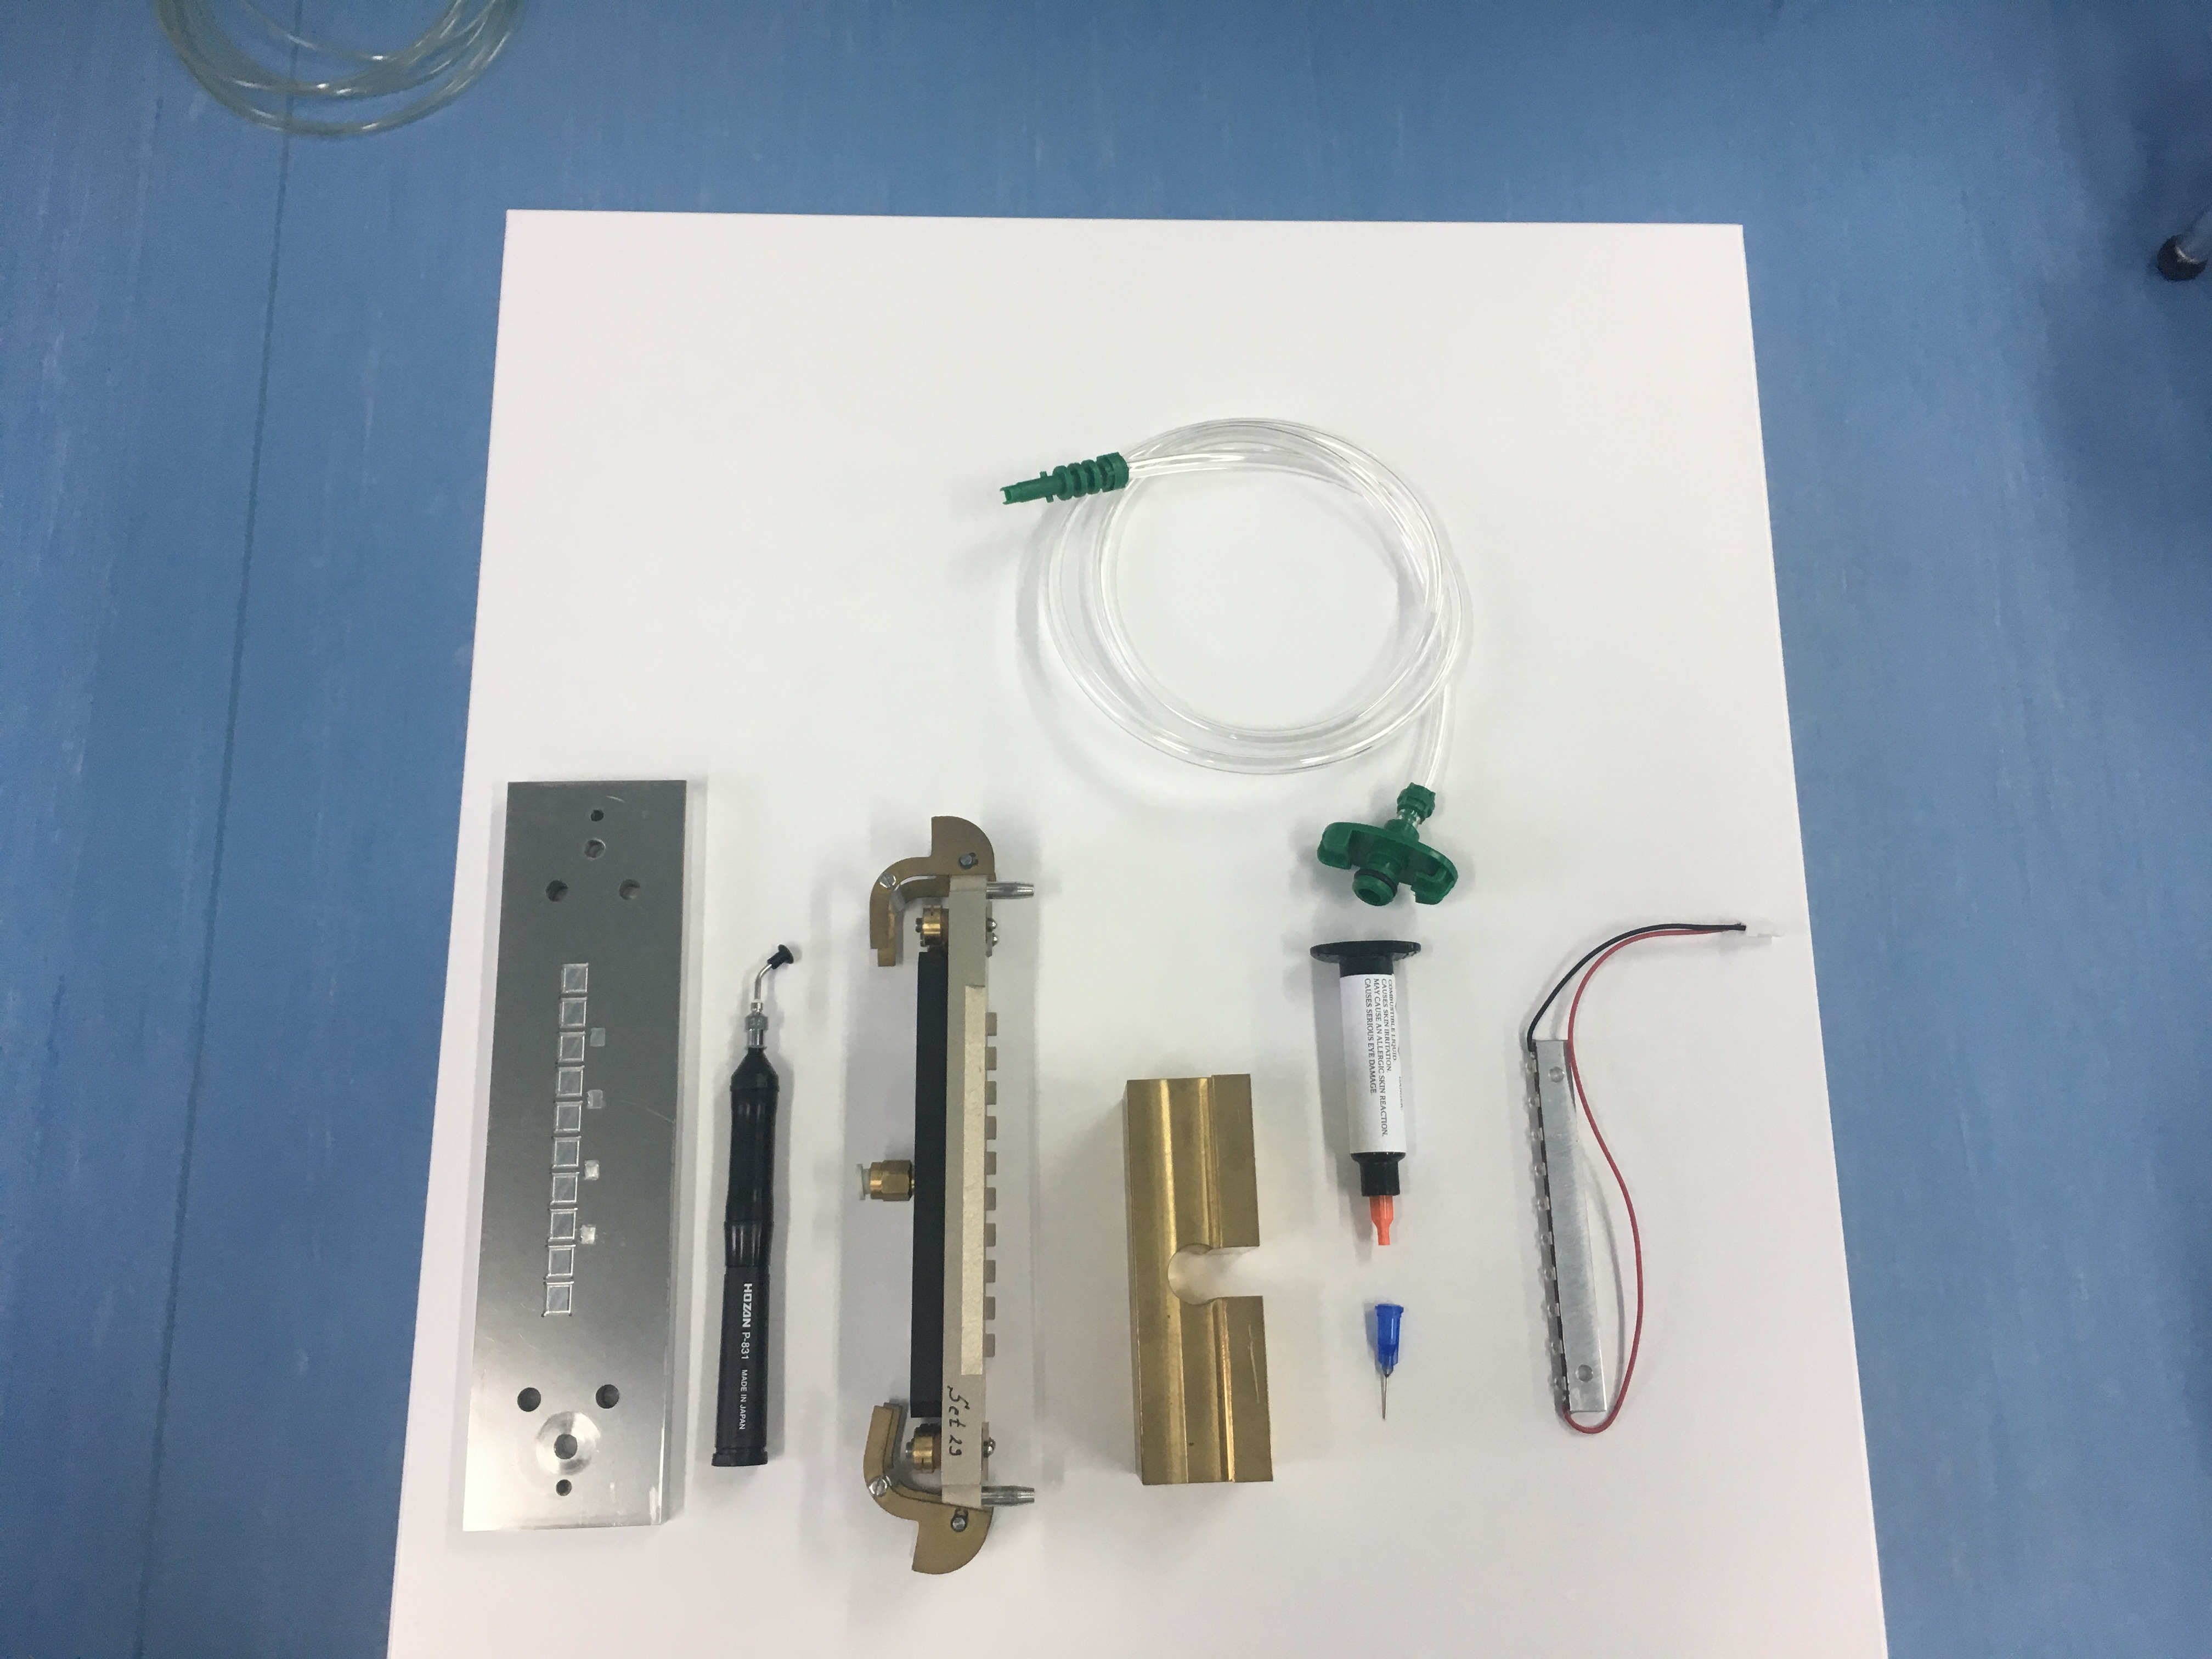
\includegraphics[width=0.7\textwidth]{img/GlueMaterials.jpg}
\caption{Materials used in the gluing process. These materials are located on the table, except for the cleaning materials which are located by the sink outside the clean room.}
\label{materials}
\end{figure}
\end{center}

\begin{itemize}
    \item Northson EPD Dispensing Robot and Dispensing Controller. 
    \item Tools placed on rack: holder, vacuum pen, pickup tool, weight, compressed air tube, syringe, needle, and UV LED strip  \ref{Nordson EFD_setup}
    \item Two vaccum pumps, vacuum gauge and valve
	\item Compressed air and reducing valve
    \item Isopropanol and cleaning clothes
    \item Power supply and UV LED strip
    \item Scale and micrometer
\end{itemize}

\begin{center}
\begin{figure}[h]
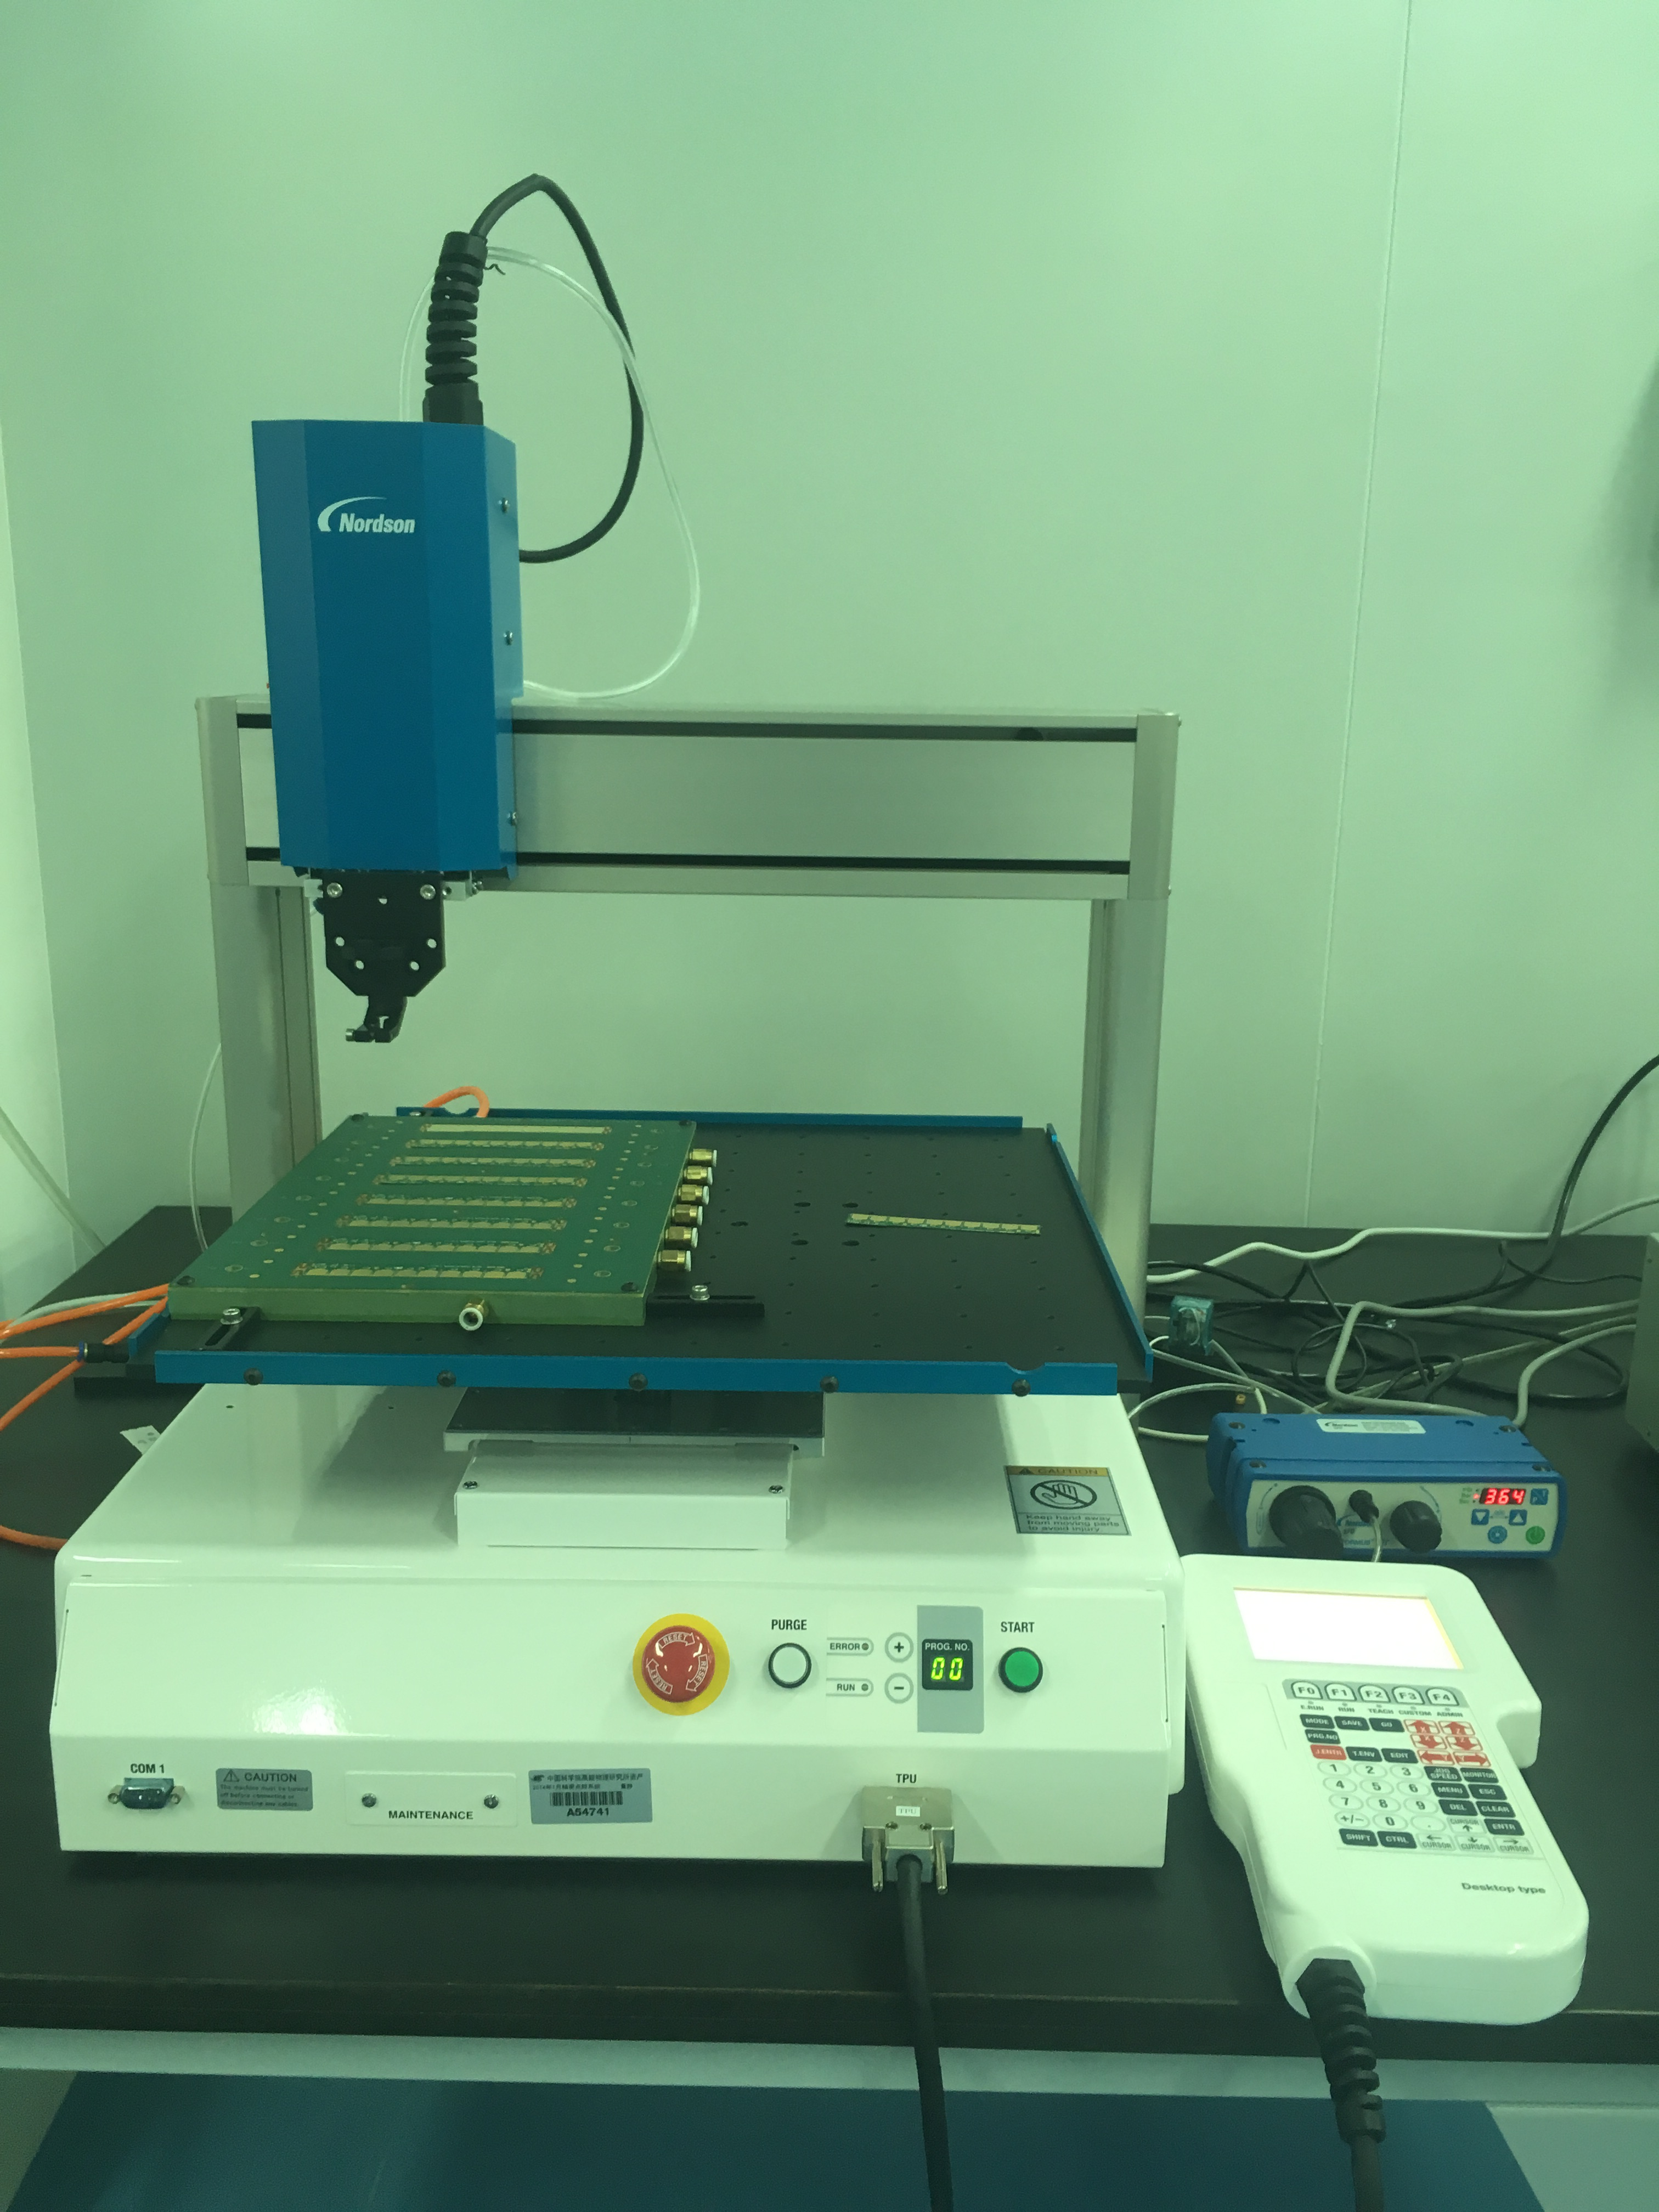
\includegraphics[width=0.7\textwidth]{img/DispensingRobot.jpg}
\caption{Nordson EFD Dispensing Robot setup. Labels indicate the main parts of the setup.}
\end{figure}
\end{center}

Note: the arrangement may vary as long as it matches the setup

%------------------------------------------------------------------
\section{Procedure}

\begin{enumerate}
    \item Perform a check of the Nordson EFD:
    \begin{enumerate}
        \item Test presence of vacuum on the gauge.
        \item Set the pressure to near 3.50 and record this value and any changes during application of the glue.
    \end{enumerate}
      \item Weigh the hybrid and ASICs on the scale so the glue mass can be calculated after application.
	\item Check the program by running it without the compressed air attached to confirm the glue will be dispensed in a 5-dot pattern above each ASIC.
    \item Dispense glue:
    \begin{enumerate}
        \item Attach vacuum tube to the hybrid holder to firmly hold hybid in place during application of the glue.
        \item Attach the compressed air tube to the top of the glue syringe and a needle to the bottom. Firmly press the syringe into the holder and tighten it in place with a hex wrench. 
        \item Run glue program and watch the glue to confirm uniform size dots of glue. If dots are uneven then clean off board with Isopropanol and apply the glue again.
    \end {enumerate}  
    \item Place the ASIC:
    \begin{enumerate}
        \item Identify the side of the ASICs with pads by inspection with a microscope for the Company's initials which will appear as a mirror image if the pads are on the bottom.
        \item Pick up the 10 ASICs with the vacuum pen and place in the ASIC holder with the pads facing up. 
        \item Place the pickup tool on top of the holder and attach the vacuum tube. 
        \item Move the pickup tool and ASICs to the hybrid platform and align the pins on the pickup tool with the platform. 
        \item Place the weight on top of the pickup tool.  
    \end{enumerate}
    \item Cure glue:
    \begin{enumerate}
        \item Connect the UV LED strip to the power supply.
        \item Place the UV LED strip pressed against the gap of the pickup tool. 
        \item Place a metal cover on top of the LED's to protect the operators vision.
        \item Supply the LED's with power at 33 Volts for 8 minutes.
        \item Repeat the UV exposure from the opposite side for 8 minutes.  
    \end{enumerate}
    \item Weigh the hybrid on the scale and subtract the mass of the hybrid and ASICs to find the amount of glue applied. Divide the glue mass by 10 and record the glue mass per ASIC.  	
\end{enumerate}


%------------------------------------------------------------------
\section{Documentation}
The following information needs to be recorded.
\begin{itemize}
    \item Date, time (start--end) and operator's name
    \item Program Number, mass, spacer size if gap adjusted, temperature
    \item List of parts used:
	\begin{itemize}
	    \item ASIC
	    \item SMD
	    \item hybrid
	\end{itemize}
\end{itemize}

Find the report at $\sim\backslash atlasitk\_assembly\backslash reports$. Any special observations, e.g. damage to parts ... Publish it in the ATLAS ITk in OneNote.....(Need to discuss before assembly production)

\end{document}

